\documentclass[tikz,border=12pt]{standalone}
\usepackage[T1]{fontenc}
\usepackage{lmodern,amsmath,amssymb}
\usetikzlibrary{arrows.meta}
\definecolor{ink}{HTML}{183444}
\definecolor{blue}{HTML}{1B6780}
\definecolor{amber}{HTML}{AD601A}
\begin{document}
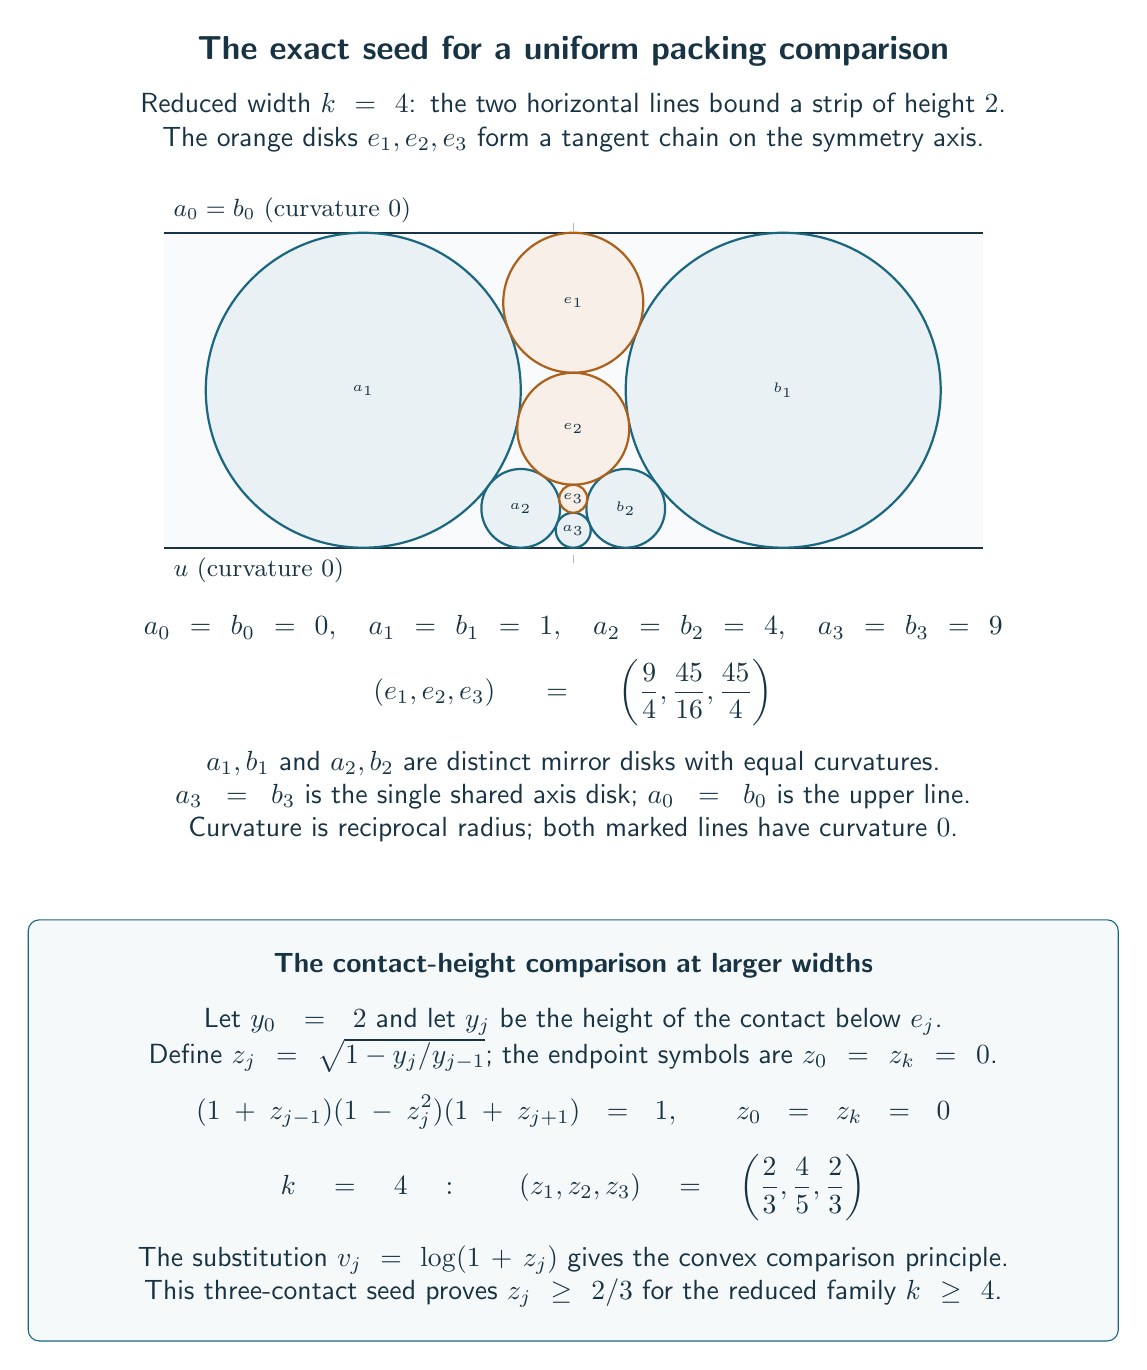
\begin{tikzpicture}[font=\sffamily,text=ink,>=Stealth]
\node[font=\sffamily\large\bfseries] at (0,6.3) {The exact seed for a uniform packing comparison};
\node[align=center,text width=13cm] at (0,5.4)
 {Reduced width $k=4$: the two horizontal lines bound a strip of height $2$.\\
 The orange disks $e_1,e_2,e_3$ form a tangent chain on the symmetry axis.};
\begin{scope}[scale=2]
\fill[blue!3] (-2.6,0) rectangle (2.6,2);
\draw[ink,thick] (-2.6,0)--(2.6,0);
\draw[ink,thick] (-2.6,2)--(2.6,2);
\draw[ink!35,dashed] (0,-.1)--(0,2.1);
\foreach \x/\y/\r/\name in {-1.333333/1/1/a_1,1.333333/1/1/b_1,-.333333/.25/.25/a_2,.333333/.25/.25/b_2,0/.111111/.111111/a_3}
 {\draw[blue,thick,fill=blue!9] (\x,\y) circle (\r);
  \node[font=\tiny] at (\x,\y) {$\name$};}
\foreach \y/\r/\name in {1.555556/.444444/e_1,.755556/.355556/e_2,.311111/.088889/e_3}
 {\draw[amber,thick,fill=amber!10] (0,\y) circle (\r);
  \node[font=\tiny] at (0,\y) {$\name$};}
\node[anchor=south west,font=\small] at (-2.6,2) {$a_0=b_0$ (curvature $0$)};
\node[anchor=north west,font=\small] at (-2.6,0) {$u$ (curvature $0$)};
\end{scope}
\node[align=center,text width=13cm] at (0,-2.3)
 {$\displaystyle a_0=b_0=0,\quad a_1=b_1=1,\quad a_2=b_2=4,\quad a_3=b_3=9$\\[6pt]
 $\displaystyle (e_1,e_2,e_3)=\left(\frac94,\frac{45}{16},\frac{45}{4}\right)$\\[8pt]
 $a_1,b_1$ and $a_2,b_2$ are distinct mirror disks with equal curvatures.\\
 $a_3=b_3$ is the single shared axis disk; $a_0=b_0$ is the upper line.\\
 Curvature is reciprocal radius; both marked lines have curvature $0$.};
\node[draw=blue,rounded corners,fill=blue!4,align=center,text width=13cm,inner sep=12pt] at (0,-7.4)
 {\textbf{The contact-height comparison at larger widths}\\[8pt]
 Let $y_0=2$ and let $y_j$ be the height of the contact below $e_j$.\\
 Define $z_j=\sqrt{1-y_j/y_{j-1}}$; the endpoint symbols are $z_0=z_k=0$.\\[8pt]
 $\displaystyle (1+z_{j-1})(1-z_j^2)(1+z_{j+1})=1,
 \qquad z_0=z_k=0$\\[8pt]
 $\displaystyle k=4:\quad (z_1,z_2,z_3)=\left(\frac23,\frac45,\frac23\right)$\\[8pt]
 The substitution $v_j=\log(1+z_j)$ gives the convex comparison principle.\\
 This three-contact seed proves $z_j\geq2/3$ for the reduced family $k\geq4$.};
\end{tikzpicture}
\end{document}
